\begin{frame}
\frametitle{AugUCB Algorithm for TBP {(Chapter 5)}}
\begin{figure}
%\caption{AugUCB Flowchart}
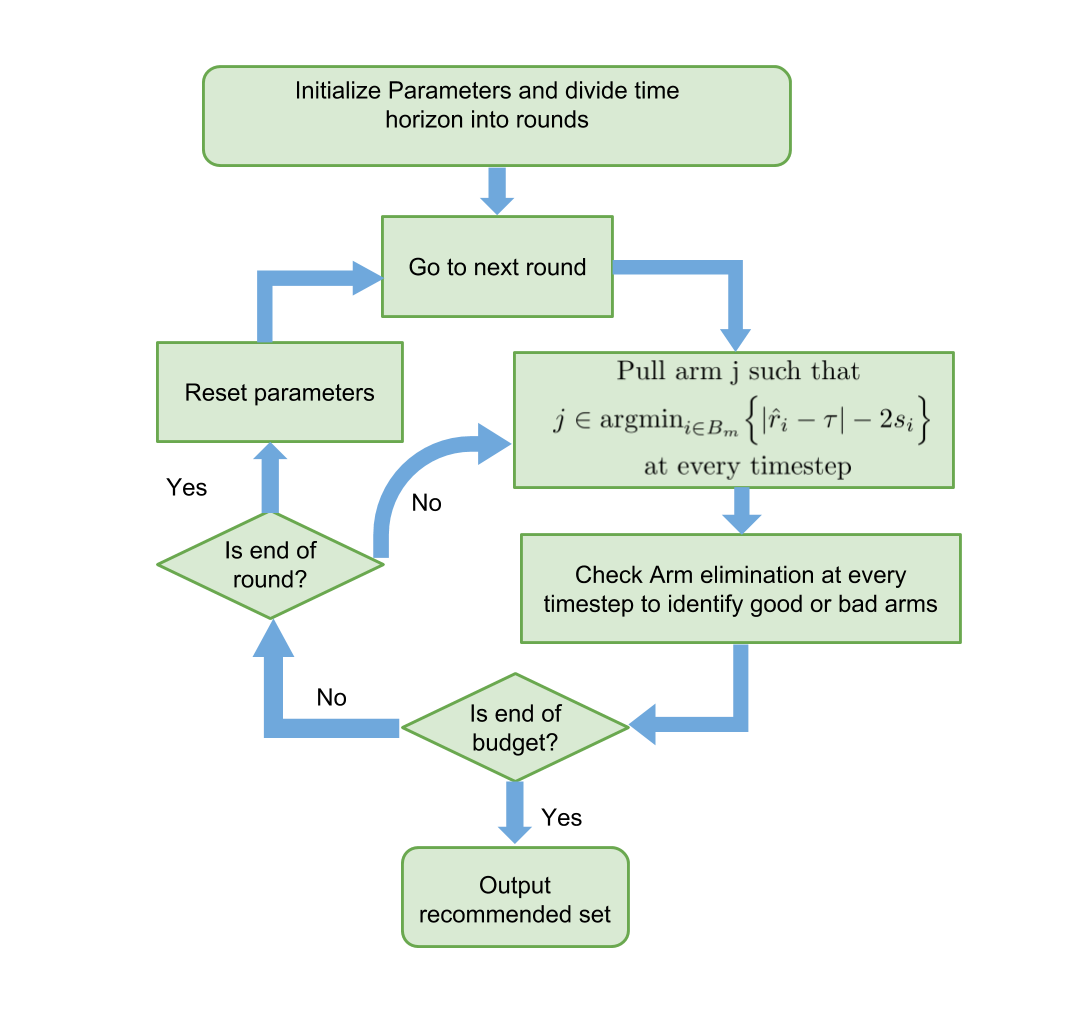
\includegraphics[scale=0.24]{img/AugUCB_flow.png}
\end{figure}
\end{frame}



%\begin{frame}
%\frametitle{AugUCB algorithm (Intuition, Arm pulling)}
%\begin{itemize}
%%\item We define $\Delta_i = |r_i - \tau| $ . 
%\item Like UCB-Imp, AugUCB also divides the time budget $T$ into rounds.
%\item At every timestep we pull arm j s.t. $j\in\argmin_{i\in B_{m}}\Big\lbrace |\hat{r}_{i} - \tau | - 2s_{i}\Big\rbrace$ (like APT). 
%\end{itemize}
%
%\begin{figure}
%%\caption{AugUCB Intuition (Arm pulling)}
%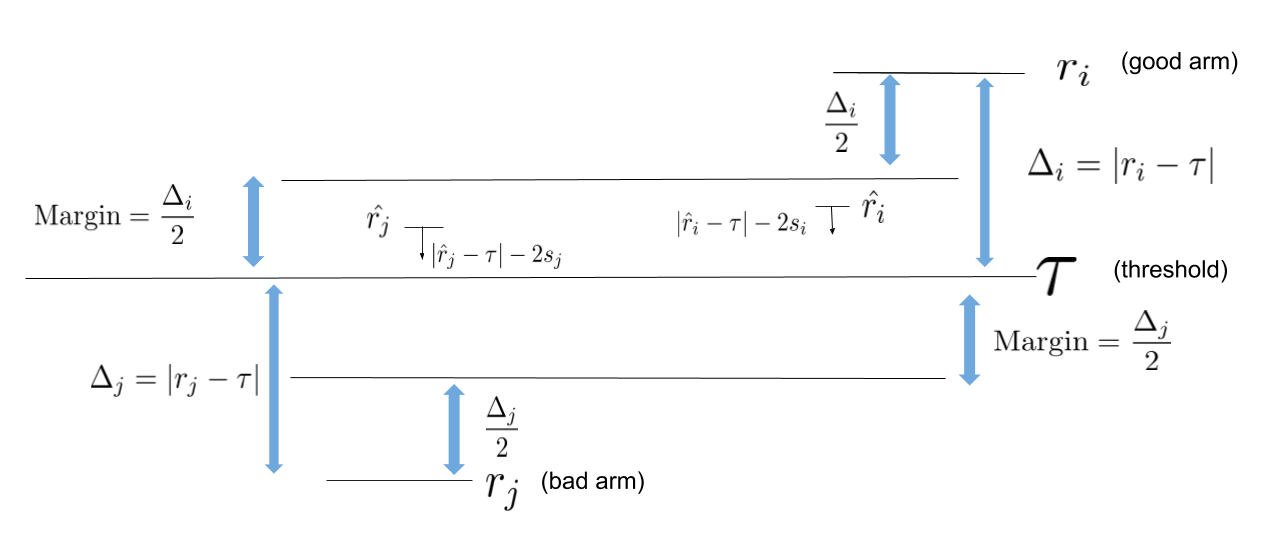
\includegraphics[scale=0.278]{img/SeminarThresholdBandit.png}
%\end{figure}
%\end{frame}
%
%\begin{frame}
%\frametitle{AugUCB algorithm (Intuition, Arm Elimination)}
%\begin{itemize}
%\item We eliminate an arm when we are sure that $\hat{r}_i$ is close to $r_i$ with high probability and hence identify it as good or bad arm.
%\item It's risky to eliminate an arm when $\hat{r}_i$ is inside \emph{Margin}. 
%\item Confidence interval $s_i$ will make sure arm $i$ is not eliminated while inside Margin with a high probability.  
%\end{itemize}
%
%\begin{figure}
%%\caption{AugUCB Intuition (Arm Elimination)}
%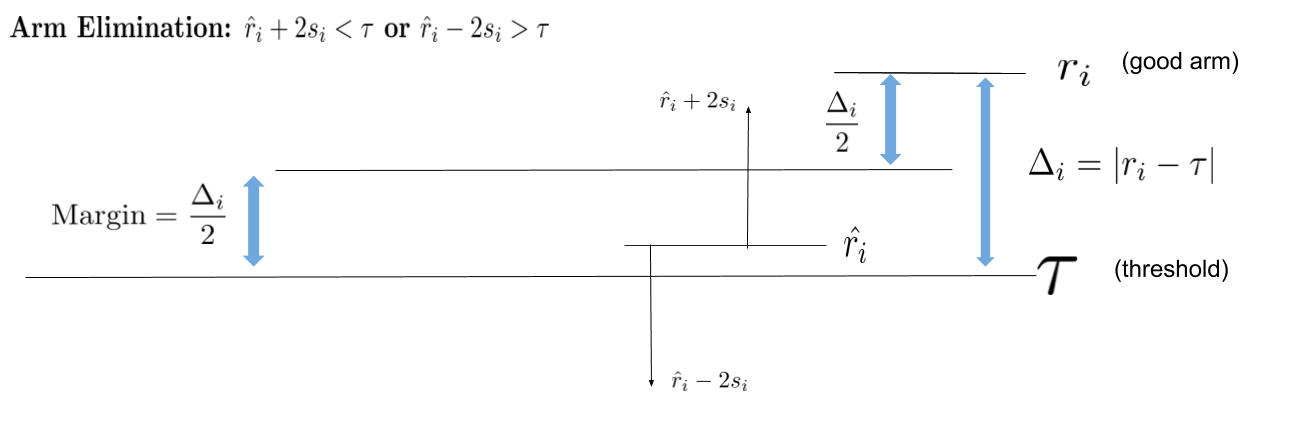
\includegraphics[scale=0.278]{img/ArmElim_1.png}
%\end{figure}
%\end{frame}
%
%\begin{frame}
%\frametitle{AugUCB algorithm (Intuition, Arm Elimination)}
%
%\begin{itemize}
%\item Now we see that $\hat{r}_i$ has moved close to its true estimate $r_i$.
%\item We eliminate $i$ and re-allocate the remaining budget to pull arms close to the threshold
%\end{itemize}
%
%
%\begin{figure}
%%\caption{AugUCB Intuition (Arm Elimination)}
%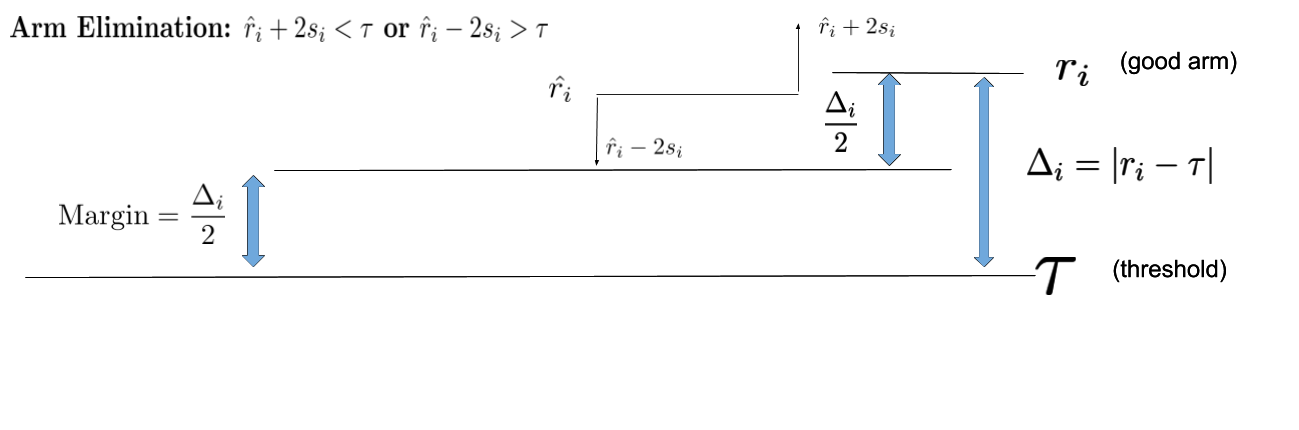
\includegraphics[scale=0.278]{img/ArmElim2.png}
%\end{figure}
%\end{frame}
%
%
%
%\begin{frame}
%\frametitle{AugUCB parameter initialization}
%\begin{figure}
%%\caption{AugUCB parameter initialization}
%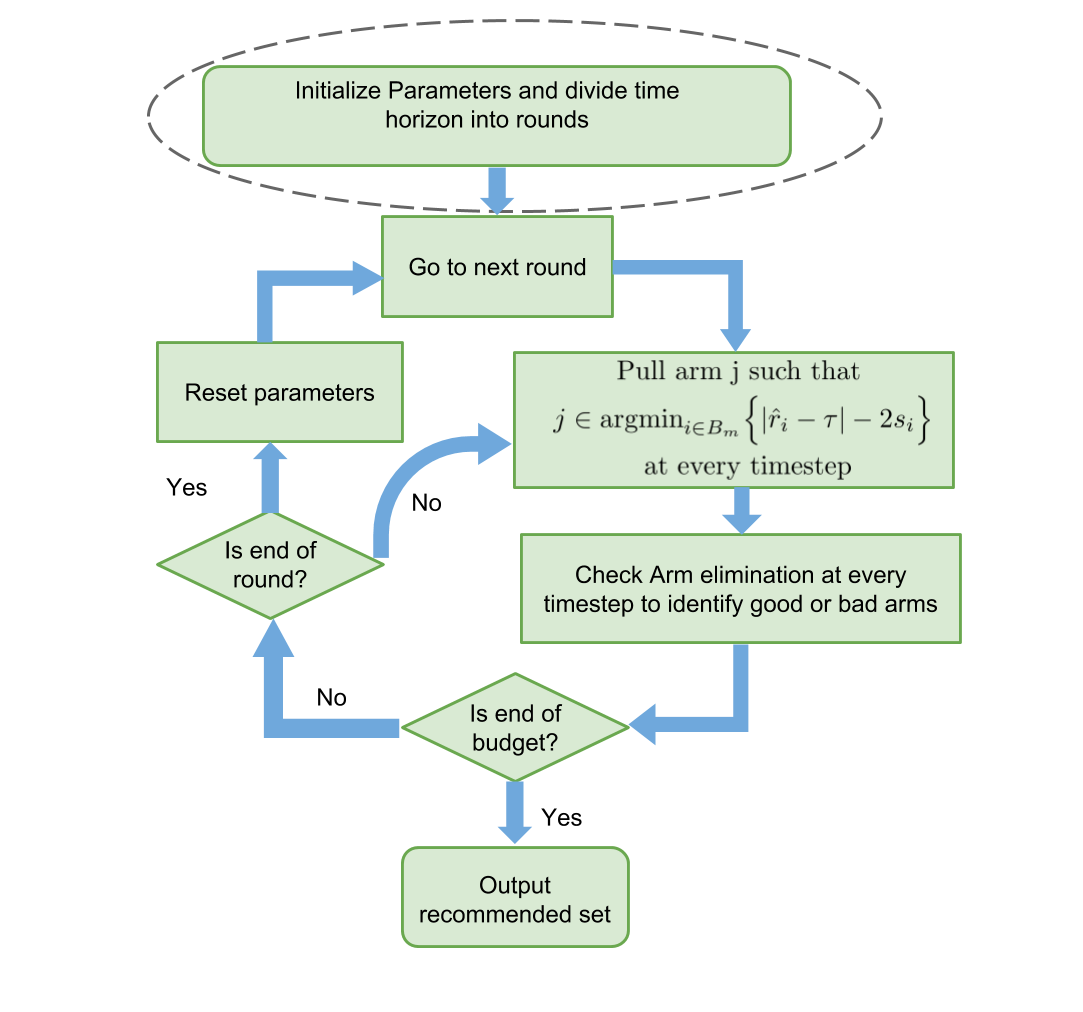
\includegraphics[scale=0.24]{img/AugUCB_flow_param.png}
%\end{figure}
%\end{frame}
%
%
%\begin{frame}
%\frametitle{Parameter initialization}
%\begin{figure}
%%\caption{AugUCB parameter initialization}
%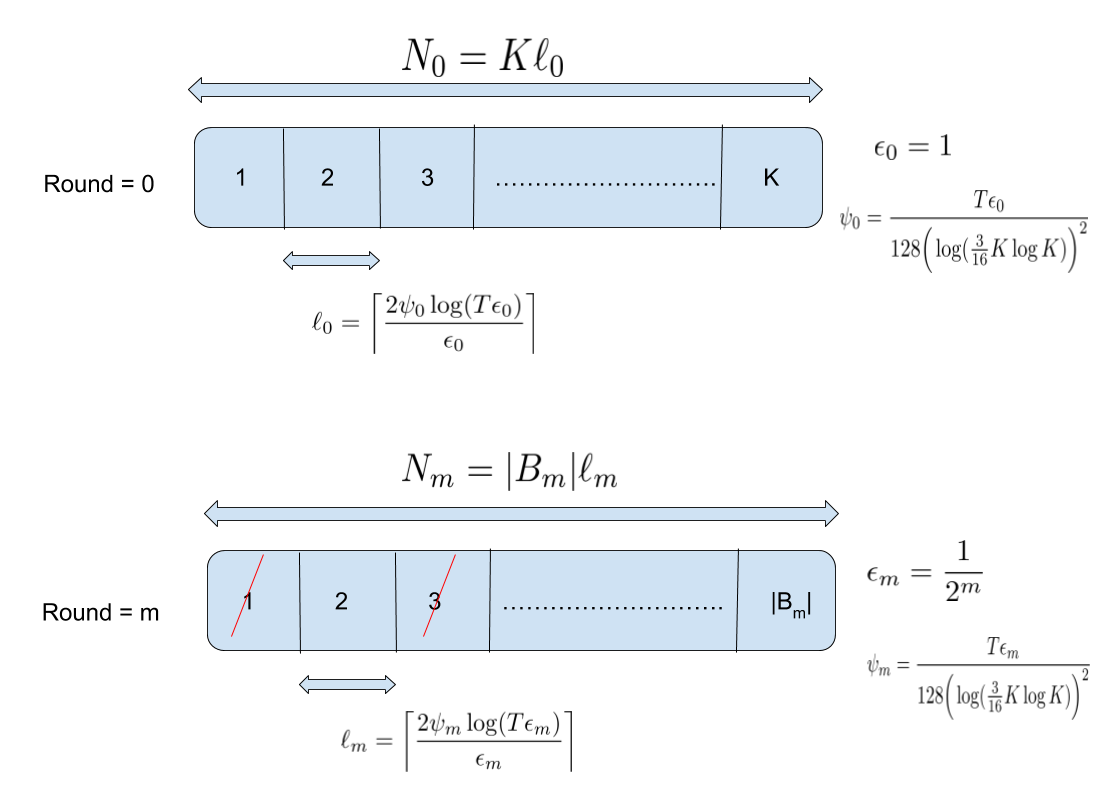
\includegraphics[scale=0.24]{img/InitReset.png}
%\end{figure}
%\end{frame}
%
%\begin{frame}
%\frametitle{AugUCB arm pull}
%\begin{figure}
%%\caption{AugUCB arm pulln}
%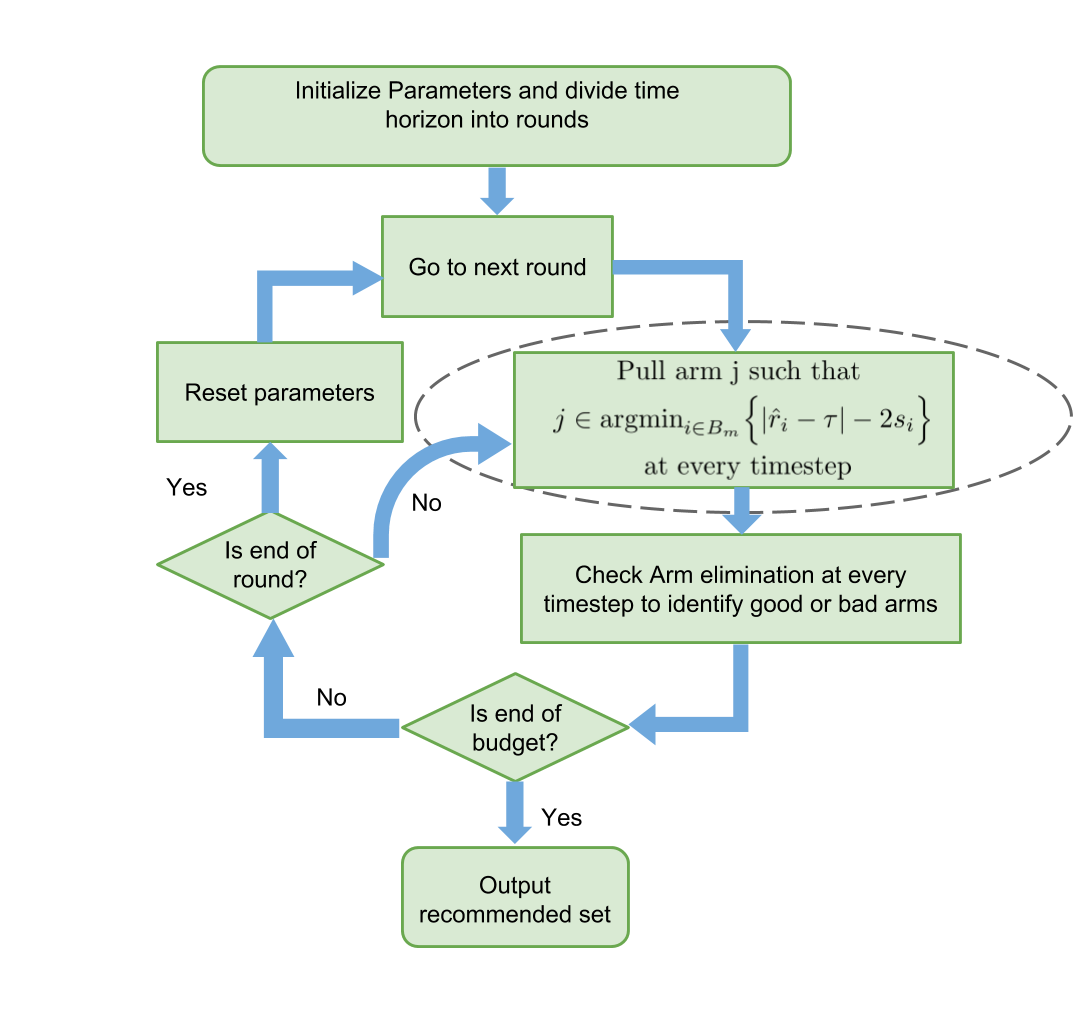
\includegraphics[scale=0.24]{img/AugUCB_flow_armpull.png}
%\end{figure}
%\end{frame}

%\begin{frame}
%\frametitle{Arm pull}
%\begin{itemize}
%\item<1-> We pull the arm that minimizes $j\in\argmin_{i\in B_{m}}\Big\lbrace |\hat{r}_{i} - \tau | - 2s_{i}\Big\rbrace$
%\item<2-> We define the confidence interval $s_i  = \sqrt{\frac{\rho\psi_m (\hat{v}_{i}+1) \log ( T \epsilon_{m})}{4 n_{i}}}$.
%\item<3-> $s_i$ decreases with more $n_i$ and $\psi_m$ and $\rho$ ensures that it decreases at a correct rate.
%\item<4-> Note that $\hat{v}_i$ estimated variance in $s_i$ makes the algorithm pull the arm which shows more variance. 
%\end{itemize}
%\end{frame}
%
%\begin{frame}
%\frametitle{AugUCB arm elimination}
%\begin{figure}
%%\caption{AugUCB arm elimination}
%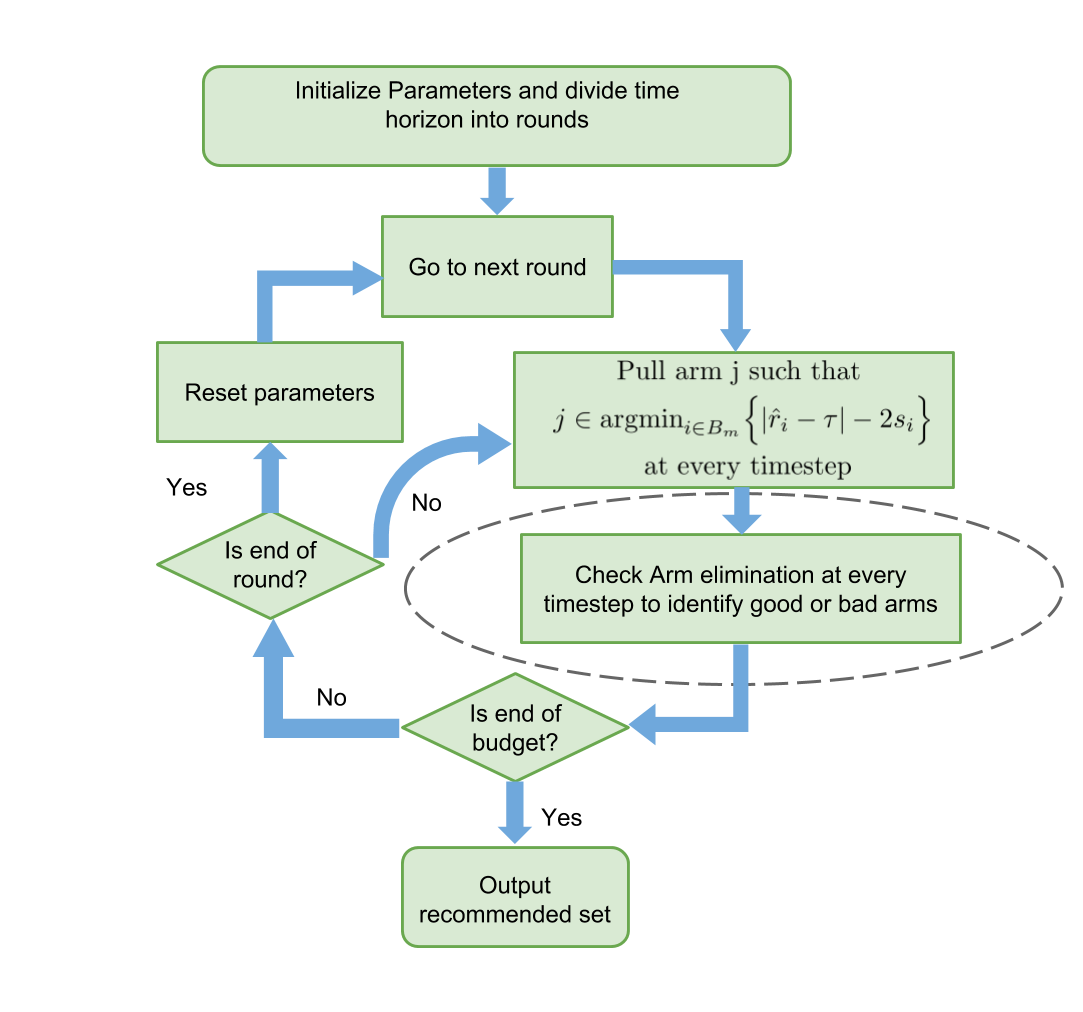
\includegraphics[scale=0.24]{img/AugUCB_flow_elim.png}
%\end{figure}
%\end{frame}
%
%
%\begin{frame}
%\frametitle{Arm elimination}
%\begin{itemize}
%\item<1-> Arm elimination condition is checked at every timestep.
%\item<2-> It identifies the arm whose estimates lies close to their true mean and thus help in identifying the good or bad arms. 
%\item<3-> It eliminates the arms which have been identified as good or bad arms (with a high probability) and re-allocates the remaining budget for surviving arms. 
%\end{itemize}
%\end{frame}
%
%
%\begin{frame}
%\frametitle{AugUCB parameter reset}
%\begin{figure}
%%\caption{AugUCB parameter reset}
%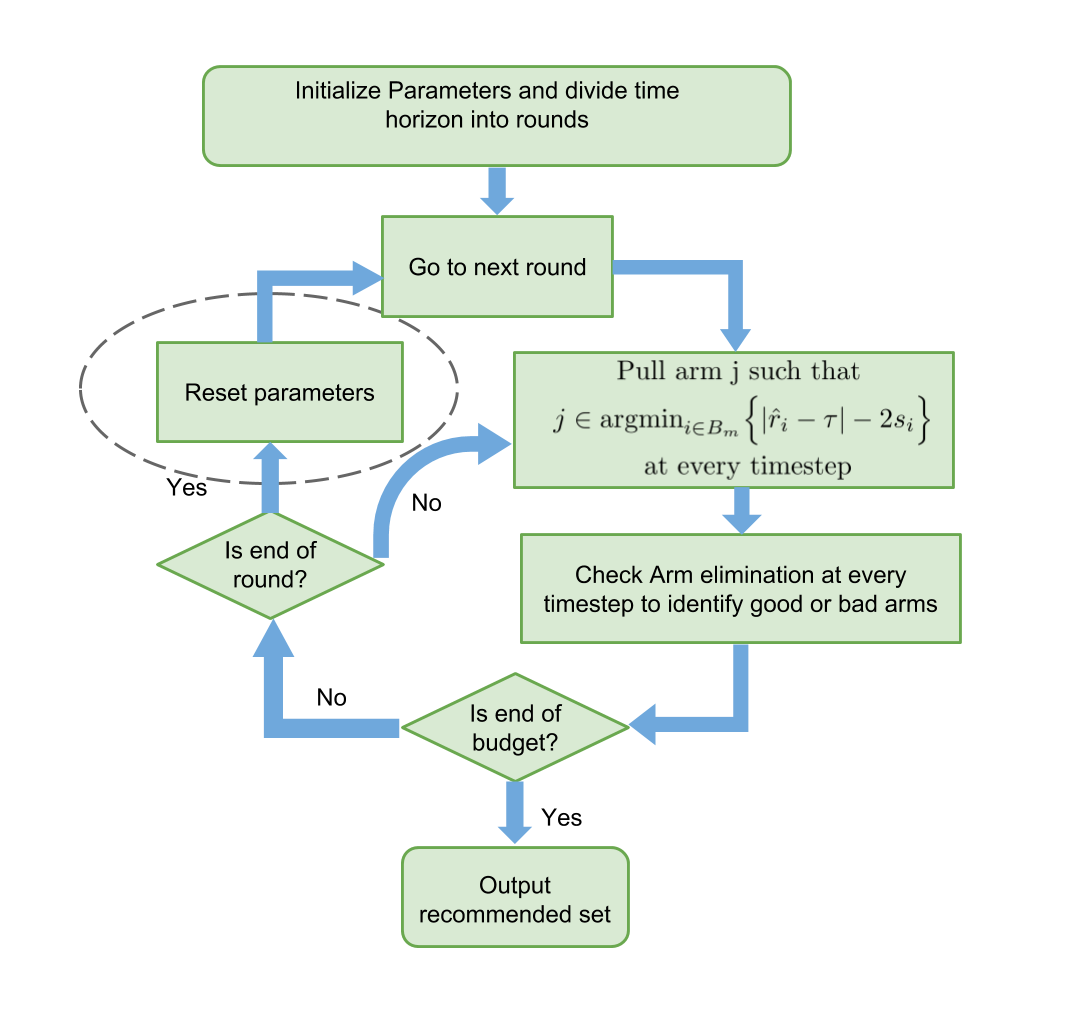
\includegraphics[scale=0.24]{img/AugUCB_flow_reset.png}
%\end{figure}
%\end{frame}
%
%
%\begin{frame}
%\frametitle{AugUCB parameter reset}
%\begin{itemize}
%\item<1-> Increase the allocated pulls $\ell_m$ for each surviving arms.
%\item<2-> Proportionally reduce the exploration factor $\psi_m$ for next round.
%%\item<2-> Recalculate the budget for each surviving arms.
%\item<3-> Recalculate the length of next round on the number of surviving arms.
%\end{itemize}
%\end{frame}
%
